\begin{frame}{Simulation 1/2}
    \inputifexists{sections/evaluation/beamernotes/sim1.tex}

    \setcounter{footnote}{0}

    \begin{itemize}
        \item Simulator built from the ground up % in Scala
        \begin{itemize}
            \item Inspired by Omega's\footnotemark{} \textit{lightweight simulator}\footnotemark{}
            \item Supports multiple resource dimensions, \glslink{resource:physical:switch}{switch resources}, and \glspl{resource:composite}
        \end{itemize}
        \item Simulated data center physical architecture: fat-tree with 4 pods
        \begin{itemize}
            \item \glslink{resource:physical:switch}{Switches} have \textit{properties} (e.g., list of supported \gls*{inp} solutions)
        \end{itemize}
        \item 3 days-long randomly-generated workload
        \begin{itemize}
            % "A thread-safe `WorkloadProvider`. Generates workloads with `Job`s that have
            % interarrival rates, numTasks, requirements and lengths sampled from exponential
            % distributions. Assumes that all tasks in a job are identical
            % (and so no per-task data is required)."
            \item Job properties (e.g., requirements, requests' interarrival time, etc.) are sampled from exponential distributions % FIXME keep this?
        \end{itemize}
        \item Simple greedy scheduler
    \end{itemize}

    \setcounter{footnote}{1}
    \footnotetext{\cite{omega}, \textsuperscript{2}available at \href{https://github.com/google/cluster-scheduler-simulator}{github.com/google/cluster-scheduler-simulator}}
\end{frame}

\begin{frame}{Simulation 2/2}
    \inputifexists{sections/evaluation/beamernotes/sim2.tex}
    \begin{itemize}
        % What's in the template database
        \item The template database contains two entries for the previously-mentioned generic groups
        \begin{itemize}
            \item In-network storage (switch chain)
            \item In-network data aggregation (switch tree)
        \end{itemize}
        % Metric and sweep
        \item Sweep: percentage of requests including \glspl{resource:composite:inp}
        % STC
        \item \gls*{stc}: the reduction of server tasks once an \gls*{inp} solution is introduced
        \vspace{3mm}
        \begin{equation*}
            \gls*{stc}=\dfrac{\#server\ tasks\ without\ \gls*{inp}}{\#server\ tasks\ with\ \gls*{inp}}
        \end{equation*}
    \end{itemize}
\end{frame}

% Results
\begin{frame}{Results 1/3}
    \inputifexists{sections/evaluation/beamernotes/res1.tex}
    \begin{figure}
        \captionsetup{font=scriptsize}
        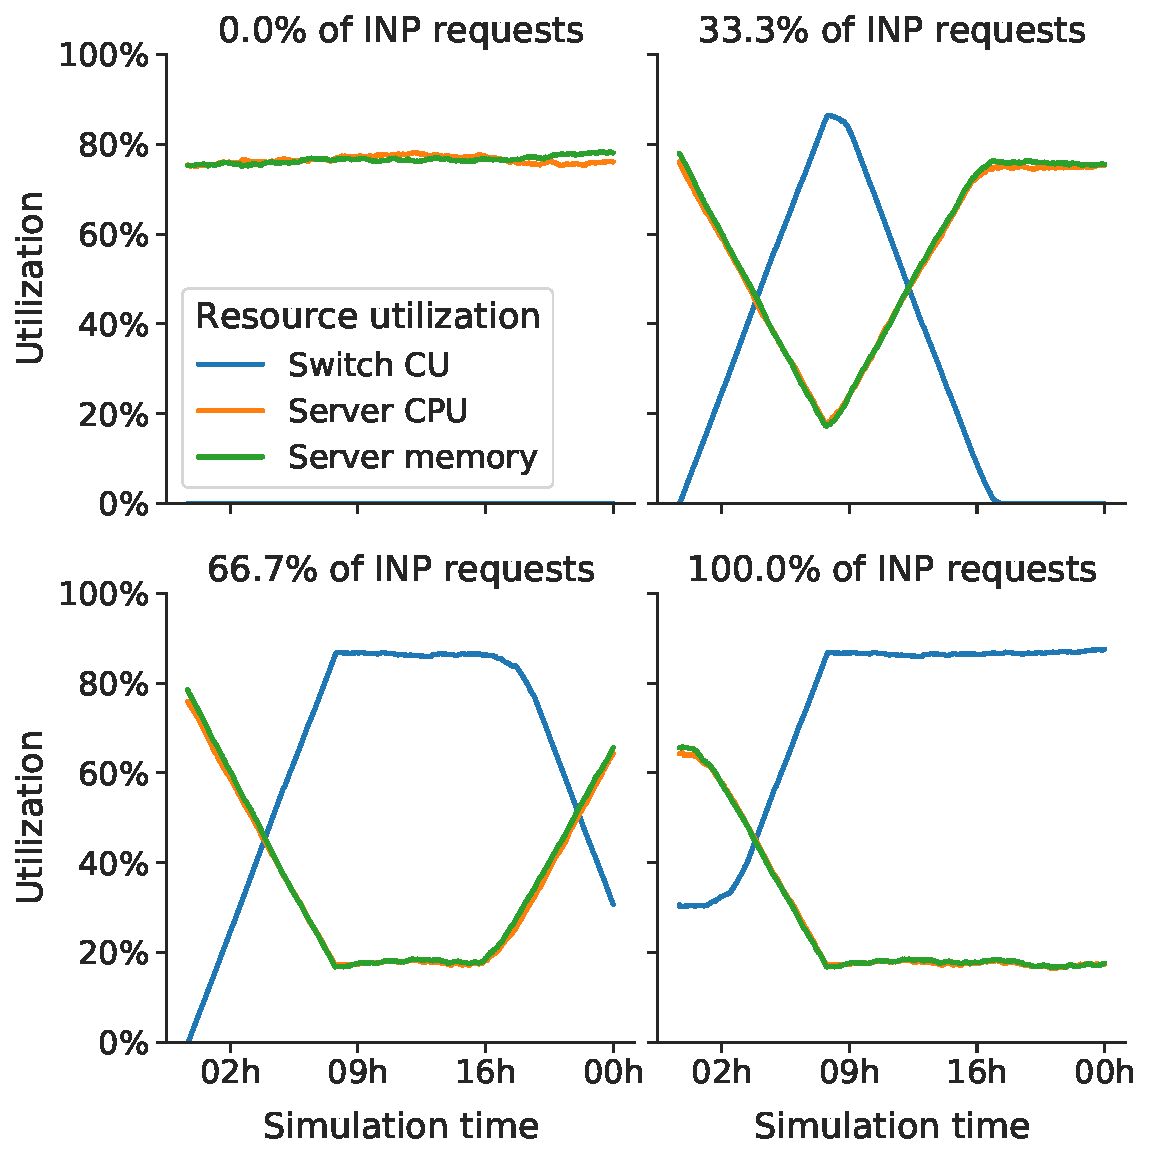
\includegraphics[page=1, width=.51\textwidth]{evaluation/results/util-multigraph.pdf}
        \caption{\gls*{resource:physical} utilization for different amounts of \gls*{inp} requests}
    \end{figure}
\end{frame}

\begin{frame}{Results 2/3}
    \inputifexists{sections/evaluation/beamernotes/res2.tex}
    \vspace{4mm}
    \begin{figure}
        \captionsetup{font=footnotesize}
        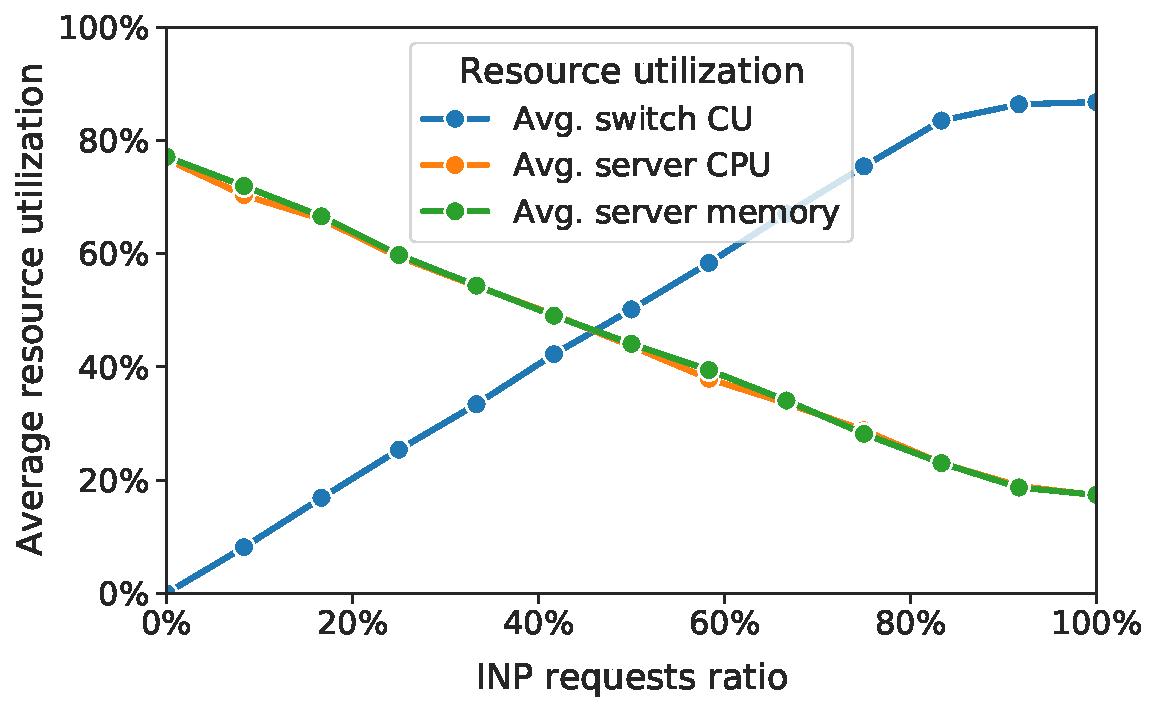
\includegraphics[page=1, width=.65\textwidth]{evaluation/results/avg-util.pdf}
        \vspace{2mm}
        \caption{Average \glslink{resource:physical}{resource} utilization as a function of the \gls*{inp} requests ratio}
    \end{figure}
\end{frame}

\begin{frame}{Results 3/3}
    \inputifexists{sections/evaluation/beamernotes/res3.tex}
    \vspace{2mm}
    \begin{figure}
        \captionsetup{font=footnotesize}
        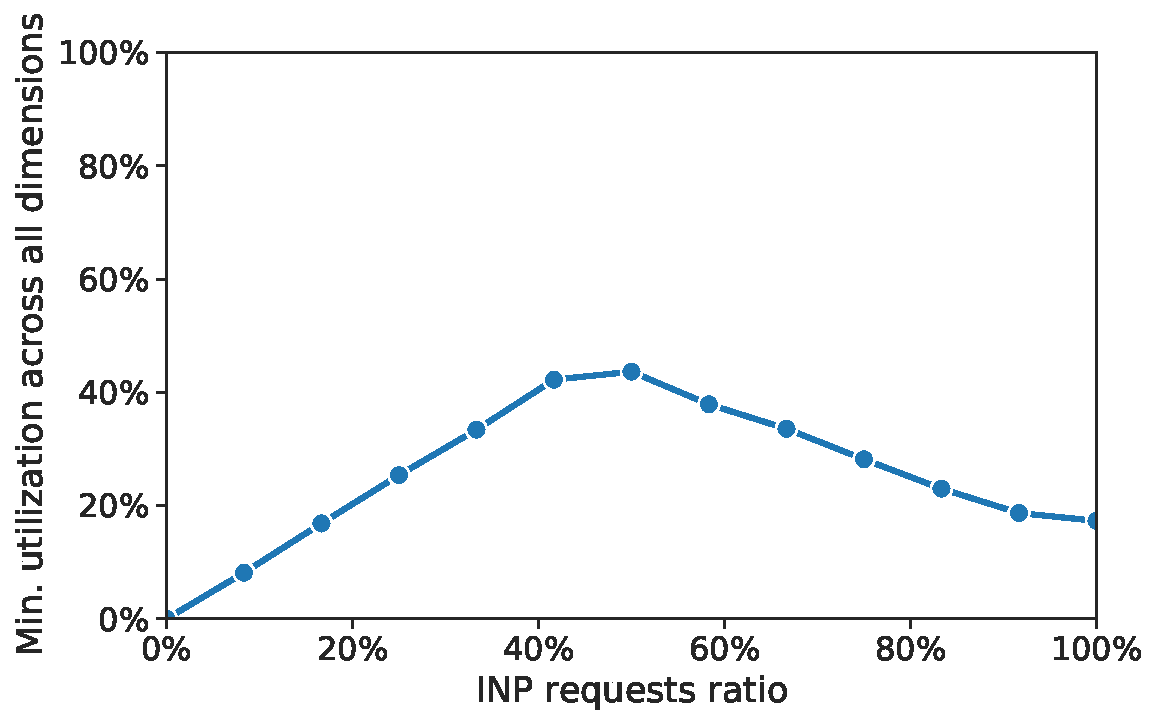
\includegraphics[page=1, width=.65\textwidth]{evaluation/results/min-util.pdf}
        \vspace{2mm}
        \caption{Minimum \glslink{resource:physical}{resource} utilization across all dimensions}
    \end{figure}
\end{frame}
